\section{Scalar field on Schwarszchild spacetime}
Although the final goal in this field is to compute tensor waveforms that can be used as templates for LISA searches, for the purposes of obtaining the desired accuracy, it is important to improve our computational methods. We do this by performing comparison studies using scalar, rather than tensor, self force methods to make the problem more tractible. I have performed the simplest of such comparison studies-- I have reimplemented Peter Diener's Fortran scalar self-force code, with a slightly modified design, in C++. The desired goal was for the results to match to within roundoff error. This was achieved for scalar fields without a source and for scalar fields with point sources on circular orbits (see Chapter~\ref{circularorbit}.


\subsection{Scalar field wave equations}
A scalar field is a field that has one one degree of freedom at a given point in space-- rather than being a matrix, it has a single value. The scalar wave equation, on a Schwarzschild background,in the absence of a source, is, in its most abstract form, the same as in flat spacetime. 
\begin{equation}
  \Box\Psi=0
\end{equation}
The details of the implementation are a little different, to account for the curvature of space. This enters through the metric. For a scalar field, the D'Alembertian can be written
\begin{equation}
  \Box\Psi=\frac{1}{\sqrt{-g}}\partial_\mu(\sqrt{-g}\partial^\mu\Psi)=0
\end{equation}
where $g$ is the determinant of $g^{\mu\nu}$.~\cite{Wald} 

\subsubsection{Multipole moment decomposition}

\subsubsection{Tortoise coordinates}
In this code, we use a mixture of tortoise (Eddington-Finkelstein) and hyperboloidal coordinates. Tortoise coordinates have the property that they go to infinity at the horizon (scri minus) and infinity at lightlike infinity (scri plus). It is beneficial to place scri minus at an unreachable distance in coordinate space so that the boundary conditions at the horizon become trivial and there is no leakage of information from the interior of the blackhole to outside the horizon in the process of discritization. It is also beneficial to increase the number of computational elements near the horizon by compactifying the coordinates there. Tortoise coordinates transform only the radial coordinate, leaving the angular and time coordinates alone.~\cite{Wald}
\begin{eqnarray}
  t_*=t\\
  r_*=r+2GM\ln|\frac{r}{2GM}-1|\\
  \theta_*=\theta\\
  \phi_*=\phi
\end{eqnarray}
We solve the wave equation in tortoise coordinates in one region of the code. I have rederived this equation in Mathematica and verified the form that appears in Peter Diener's Fortran scalar self-force code. The wave equation in tortoise coordinates is
\begin{equation}
  \frac{d^2\psi}{dt^2}=\frac{d^2\psi}{dr_*^2}-\frac{1}{r^5}(\frac{2M}{r}+(l+1)l)(1-\frac{2M}{r})\psi
\end{equation}
$r$ is in Schwarszchild coordinates, $r_*$ is in tortoise coordinates, $l$ is the spherical harmonic l-mode (discussed below), which accounts for the angular dependence, and $\psi$ is a function of tortoise coordinates.


\subsubsection{Hyperboloidal coordinates}  
Hyperboloidal coordinates are necessary; however, because infinities are computationally unreachable. It is clear that space infinitessimally close to the horizon is important, since the curvature of space is strongest there, and it is still causally connected to the exterior region. To make the horizon reachable in a finite number of computational elements, while retaining the property that more computational elements are placed near the horizon than far away, hyperboloidal coordinates are introduced in the region closest to the horizon. In a middle region, tortoise coordinates are used. In the region furthest from the blackhole, hyperboloidal coordinates are used again to place scri plus at a finite number, yet maintaning the property that fewer computational elements are needed far away from the blackhole. Hyperboloidal coordinates are described by the transformation~\cite{hyperboloidalCoordinates}

There are a few key features. The angular coordinates are not transformed. The time coordinate preserves the stationarity of the background metric, and thus the new time variable, $\tau$, must be related to the old time variable, $t_*$, by an offset dependent only upon $r_*$, $\tau=t-h(r_*)$. For ingoing waves in the inner region, $t-r_*=\tau-\rho$ and in the outgoing region, $t+r_*=\tau+\rho$ to preserve the structure of the light cone. Bernuzzi, Nagar, and Zenginoglu define $H=\frac{dh}{dr_*}$. They introduce a compactification that depends on a window function $\Omega$~\cite{OmegaTransferFunction}, such that the tortoise radius gets redefined  $r_*=\frac{\rho}{\Omega(\rho)}$, resulting in an expression for the height function $H$ in terms of the hyperboloidal radius,  $H(\rho)=1-\frac{\Omega^2}{\Omega-\rho\Omega^\prime}$. Their final wave equation, for ingoing waves, is~\cite{hyperboloidalCoordinates}
  \begin{eqnarray}
    \partial_t^2-\partial_{r_*}^2=-(1-H^2)\partial_\tau^2\nonumber\\
    +(1-H)(-2H\partial_\tau\partial_\rho+(1-H)\partial_\rho^2-(\partial_\rho H)(\partial_\tau+\partial_\rho))
  \end{eqnarray}    
I have verified this equation, and derived the outgoing wave equation, in Mathematica.

  



\subsubsection{Initial conditions and boundary conditions}
Since there is no source for the scalar field in the C++ code, it must be set to some initial value and allowed to fall into the blackhole or radiate away its energy to infinity. A gaussian initial condition in the time derivative of the scalar field, centered at computational coordinate zero (which was some physical distance outside the black hole horizon), was chosen.   

Boundary conditions were matched automatically by the coordinate transformation between tortoise and hyperboloidal layers. At scri minus and scri plus, the boundary conditions were that the scalar field be set to zero. 



\section{Theoretical expectations}

quasinormal modes
tails

\section{Comparison of C++ code to Fortran code}
round off noise
truncation error

\begin{figure}
  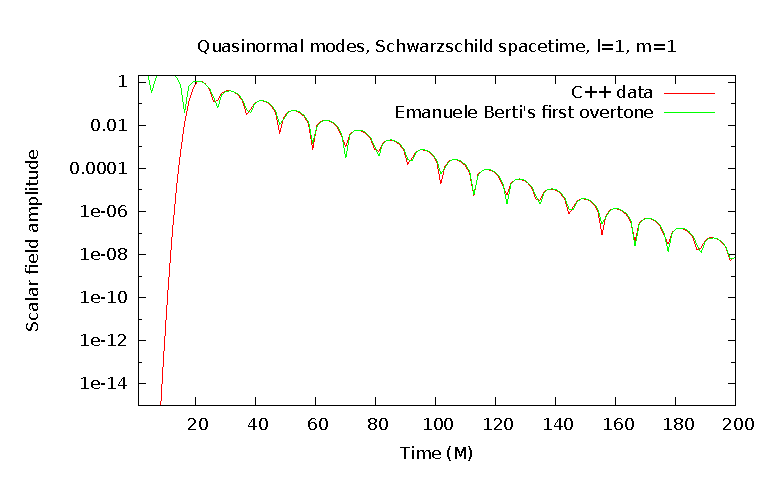
\includegraphics{l1m1qnm}
  \caption{Quasinormal mode for l=1,m=1}
  \end{figure}

\begin{figure}
  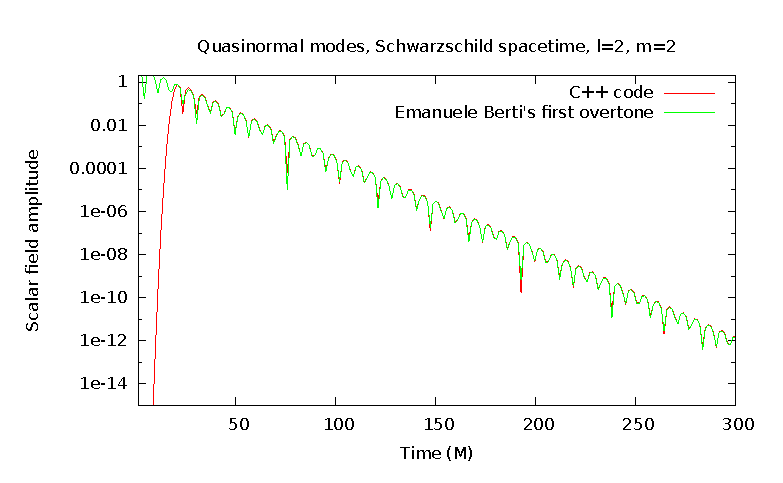
\includegraphics{l2m2qnm}
  \caption{Quasinormal mode for l=2, m=2}
\end{figure}

\begin{figure}
  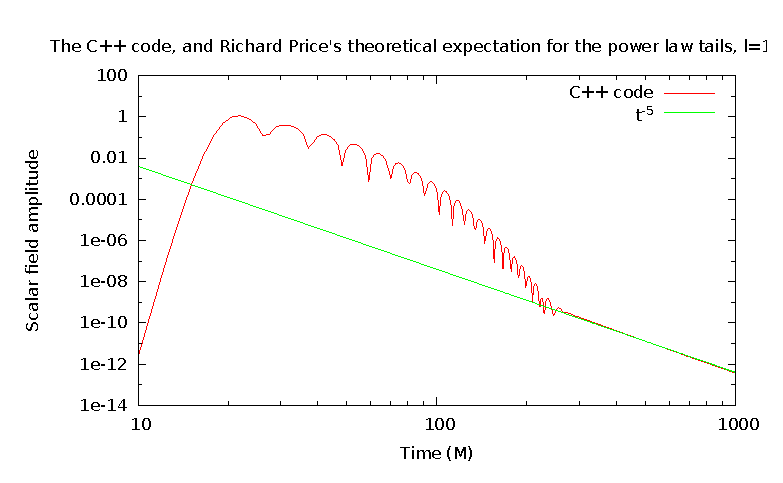
\includegraphics{l1m1tail2}
  \caption{Power law tail, l=1, m=1}
\end{figure}

\begin{figure}
  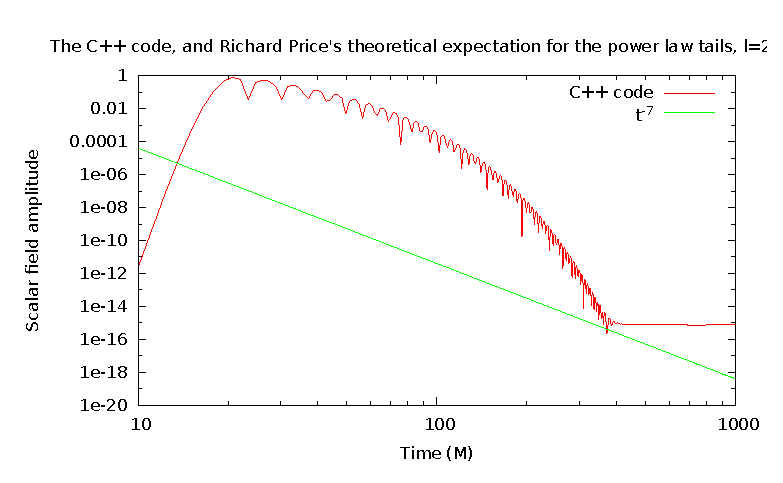
\includegraphics{l2m2tailfail2}
  \caption{Power law tail does not match expectations due to truncation error in DG method, l=2, m=2}
\end{figure}

\begin{figure}
  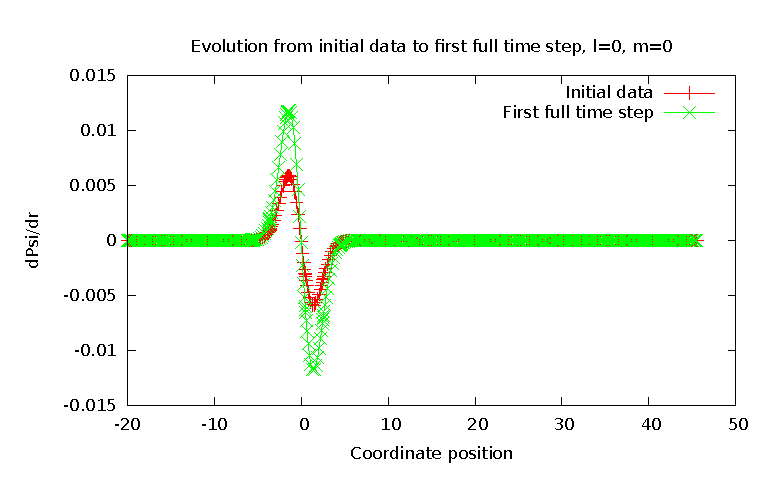
\includegraphics{phi1dl0}
  \caption{Scalar field spatial slice initial condition and first full timestep for l=0.}
\end{figure}

\begin{figure}
  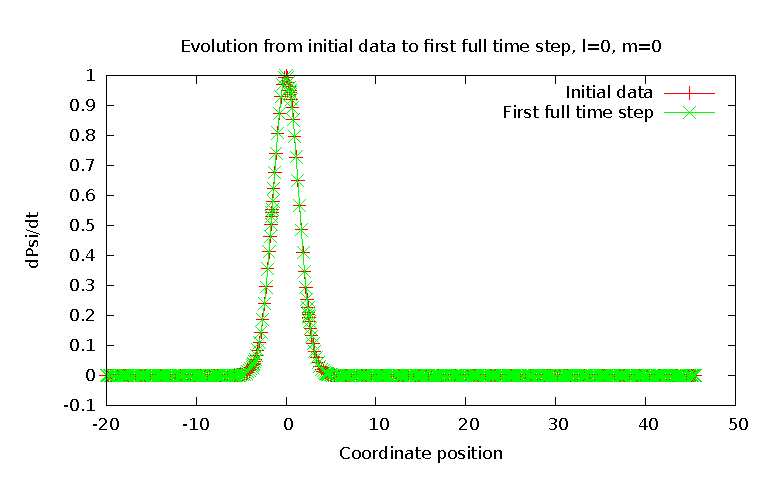
\includegraphics{rho1dl0}
  \caption{Time derivative of the scalar field spatial slice initial condition and first full timestep for l=0.}
\end{figure}

\begin{figure}
  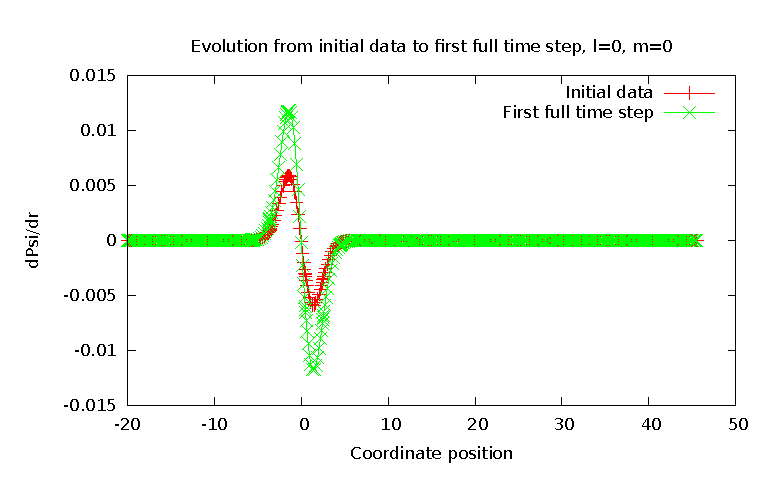
\includegraphics{phi1dl0}
  \caption{Radial derivative of the scalar field spatial slice initial condition and first full timestep for l=0.}
\end{figure}
